\section{Réalisation}
Dans cette partie, nous allons nous intéresser à plusieurs réseaux de neurones
en étudiant pour chacun en quoi son comportement peut être assimilé à une 
décision.


\subsection{Premier réseau de neurones}
\paragraph{}
Ce premier réseau \ref{reseau1} n'est constitué que de six neurones. Les deux
premiers neurones (N1 et N2) se chargent de recevoir les stimuli. Ensuite ils 
vont à la fois activer un neurone qui aura pour tâche de déclencher une 
action et un neurone qui se chargera d'inhiber l'autre branche. 

\begin{figure}[!h]
  \begin{center}
    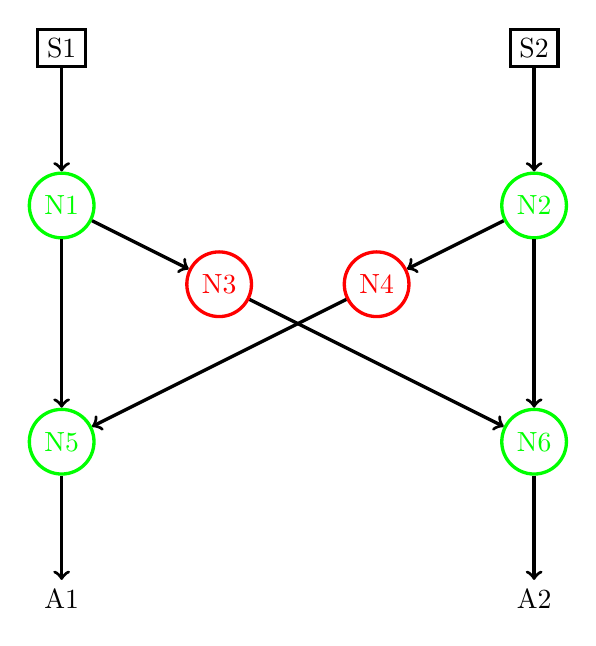
\begin{tikzpicture}[scale=0.5]
 \tikzset{directed/.style={->}} 
  \node[] (A1) at (0,0) {A1};
  \node[] (A2) at (12,0) {A2};
  \node[draw, circle, very thick, color=green] (N1) at (0,10) {N1};
  \node[draw, circle, very thick, color=green] (N2) at (12,10) {N2};
  \node[draw, circle, very thick, color=red] (N3) at (4,8) {N3};
  \node[draw, circle, very thick, color=red] (N4) at (8,8) {N4};
  \node[draw, circle, very thick, color=green] (N5) at (0,4) {N5};
  \node[draw, circle, very thick, color=green] (N6) at (12,4) {N6};
  \node[draw, very thick] (S1) at (0,14) {S1};
  \node[draw, very thick] (S2) at (12,14) {S2};
  \draw[very thick, directed] (S1) -- (N1);
  \draw[very thick, directed] (S2) -- (N2);
  \draw[very thick, directed] (N1) -- (N3);
  \draw[very thick, directed] (N2) -- (N4);
  \draw[very thick, directed] (N3) -- (N6);
  \draw[very thick, directed] (N4) -- (N5);
  \draw[very thick, directed] (N1) -- (N5);
  \draw[very thick, directed] (N2) -- (N6);
  \draw[very thick, directed] (N5) -- (A1);
  \draw[very thick, directed] (N6) -- (A2);
\end{tikzpicture}

  \end{center}
  \caption{Un réseau de neurones minimum (En vert les neurones stimulants, en rouge les inhibiteurs)}
  \label{reseau1}
\end{figure}

\paragraph{}
En fonction des stimuli reçus, ce réseau va bien prendre la décision 
d'envoyer soit l'action A1, soit l'action A2. Cependant le 
stimuli S1 conduira toujours à l'action A1 et le stimuli S2 à 
l'action A2.

Ceci est problématique car le comportement du réseau ne peut donc pas 
être assimilé à une prise de décision.

\subsection{Deuxième réseau de neurones}
\paragraph{}
En ajoutant une arête entre le S1 et N2 et une autre entre S2 et N1, cela
permet d'éviter que le stimulus 1 conduise toujours à l'action 1 et que le
stimulus 2 conduise à l'action 2. Le choix de l'action en fonction du stimulus
va dépendre des poids des connexions entre les stimuli et les deux premiers
neurones N1 et N2.

\paragraph{}
Dans le cas où on reçoit le stimulus 1, si la connexion entre N1 et S1 est
plus forte que la connexion entre N2 et S1 alors l'action 1 est choisie. 
Par contre si la connexion entre N1 et S1 est plus faible que celle entre 
N2 et S2 alors l'action 2 est effectuée. Le même raisonnement peut être 
appliqué au stimulus 2.

\begin{figure}[!h]
  \begin{center}
    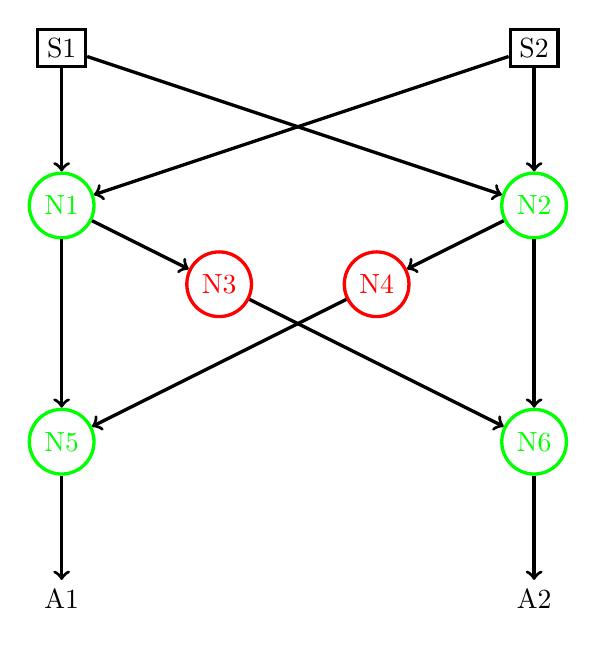
\begin{tikzpicture}[scale=0.5]
 \tikzset{directed/.style={->}} 
  \node[] (A1) at (0,0) {A1};
  \node[] (A2) at (12,0) {A2};
  \node[draw, circle, very thick, color=green] (N1) at (0,10) {N1};
  \node[draw, circle, very thick, color=green] (N2) at (12,10) {N2};
  \node[draw, circle, very thick, color=red] (N3) at (4,8) {N3};
  \node[draw, circle, very thick, color=red] (N4) at (8,8) {N4};
  \node[draw, circle, very thick, color=green] (N5) at (0,4) {N5};
  \node[draw, circle, very thick, color=green] (N6) at (12,4) {N6};
  \node[draw, very thick] (S1) at (0,14) {S1};
  \node[draw, very thick] (S2) at (12,14) {S2};
  \draw[very thick, directed] (S1) -- (N1);
  \draw[very thick, directed] (S1) -- (N2);
  \draw[very thick, directed] (S2) -- (N1);
  \draw[very thick, directed] (S2) -- (N2);
  \draw[very thick, directed] (N1) -- (N3);
  \draw[very thick, directed] (N2) -- (N4);
  \draw[very thick, directed] (N3) -- (N6);
  \draw[very thick, directed] (N4) -- (N5);
  \draw[very thick, directed] (N1) -- (N5);
  \draw[very thick, directed] (N2) -- (N6);
  \draw[very thick, directed] (N5) -- (A1);
  \draw[very thick, directed] (N6) -- (A2);
\end{tikzpicture}

  \end{center}
  \caption{Un réseau de neurones minimum (En vert les neurones stimulants, en rouge les inhibiteurs)}
  \label{reseau2}
\end{figure}

\paragraph{}
Avec ce réseau les stimuli peuvent conduire à n'importe quelle des deux
actions. Une fois les poids établis, le réseau enverra toujours les mêmes
actions en réponse aux stimuli données.
